\section{Method}
\label{sec:method}
In this study, 
we essentially follow Heimisson et al. \cite{Elias_2021, Elias_Shengduo_2022} for theoretical and numerical modeling of dynamic fault slip.
\subsection{Governing equations}
The governing equations for the poroelastic solid bulk are
\begin{align}
    Gu_{i,kk}+\frac{G}{1-2\nu}u_{k,ki}&=\alpha p_{,i} \label{eq:poro1}\\
    \frac{1}{M}p_{,t}-\kappa p_{,kk}&=-\alpha u_{k,kt} \label{eq:poro2}, 
\end{align}
where $G$ and $\nu$ are elastic shear modulus and Poisson's ratio in drained condition.
$M$ and $\alpha$ are poroelastic Biot modulus and Biot coefficient, 
respectively.
$\kappa$ is the mobility of fluid in porous medium. 
The apparent fluid diffusivity from (\ref{eq:poro2}) is $c = M \kappa$. 
However, 
since $u$ on the right hand side of (\ref{eq:poro2}) is coupled with $p$, 
the apparent $c$ does not directly reflect the diffusion of fluid content. 
Through a change of variable, 
the actual fluid diffusion for the fluid mass content $\zeta$ is given by \cite{Rice_1998_notes}
\begin{align}
    \zeta_{,t} - c_{mass} \zeta_{, kk} = 0 \label{eq:massDiffusion}, 
\end{align}
where $c_{mass}$ is given by 
\begin{align}
    c_{mass} = c \frac{K_d+\frac{4}{3} G}{K_u + \frac{4}{3} G} \label{eq:cmass}. 
\end{align}
In (\ref{eq:cmass}), 
$K_d$ and $K_u$ are drained and undrained bulk modulus, 
respectively. 
In addition to poroelastic bulk, 
in this study, 
we consider elastic but permeable bulk to further compare the poroelastic effects with solely bulk fluid diffusion.
The governing equations for elastic permeable bulk are 
\begin{align}
    Gu_{i,kk}+\frac{G}{1-2\nu}u_{k,ki}&=0 \label{eq:elastic1}\\
    p_{,t} - c p_{,kk}&= 0\label{eq:elastic2}, 
\end{align}
where $c$ is the bulk diffusivity associated with the elastic permeable bulk. 
Note that for elastic permeable solid, 
since (\ref{eq:elastic2}) is independent of $u$, 
the apparent diffusivity coincides with the mass diffusivity, i.e., 
$c_{mass} = c$. 

\subsubsection{Frictional shear layer}
Then for the shear layer, 
rate and state friction model is given by (\ref{eq:RSF1}, \ref{eq:RSF2}). 
By setting $\dot{\theta} = 0$, 
one can obtain the steady-state friction relation as
\begin{align}
    \theta_{ss} &= \frac{D_{RS}}{V} \label{eq:thetaSS} \\
    \tau_{ss}(V) &= \sigma_{eff}\left[f_* + (a-b)\log\left(\frac{V}{V_*}\right) \right] \label{eq:RSss}, 
\end{align}
and the fault is considered rate-strengthening, 
if $a-b>0$ because steady state friction increases with slip rate. 
Similarly,
the fault is considered rate-weakening if $a-b<0$.
There is a minimum slip zone size for dynamic events to nucleate \cite{ruina_slip_1983}. 
\begin{align}
    L_{slip}\ge L_{nu} \propto \frac{GD_{RS}}{(b-a)(\sigma_n-p)} \label{eq:Lnu}.
\end{align}

Besides friction,
fluid mass transport within the shear layer as well as between the shear layer and the bulk also affects the slip. 
Figure~\ref{fig:poroshear1} lists the variables involved in this problem, 
where $\delta_p^+, \delta_p^-, \delta p_c$ are the fluid pore pressure change above, 
below and in the middle of the layer, 
respectively. 
$\delta_x, \delta_y$ are fault slip and opening, 
$\kappa, \kappa_{cx}, \kappa_{cy}$ are fluid mobilities in the bulk, 
in $x$ direction of the layer, 
in $y$ direction of the layer, 
respectively. 
Based on the modeling of (Elias et al., 2022) \cite{Elias_Shengduo_2022}, 
one can get the governing equation of $\delta p_m, \sigma$ and $\theta$ as following:
\begin{align}
    \delta p_m + \frac{\beta_f^\sigma - \beta_\phi^\sigma}{\beta_f^p+\beta^p_\phi}\sigma = \frac{1}{\phi_*(\beta_f^p+\beta^p_\phi)}\left(
    \frac{Q(X,t)}{\rho_{f*}}-\phi^{pl}+\int_0^t\frac{\kappa_{cy}}{h^2}\left(\frac{1}{2}(\delta p^+ + \delta p^-)- \delta p_c\right)+\kappa_{cx}\frac{\partial^2 \delta p_m}{\partial x^2} dt'
    \right) \label{eq:layerControl1}, 
\end{align}
where $\delta p_m =\frac{1}{2}\left(\frac{1}{2}(\delta p^++ \delta p^-)+\delta p_c\right)$
is the average pore pressure change within the fault shear layer, 
through piecewise linear approximation.
$\phi_*, \rho_{f*}$ are constants of reference porosity and fluid mass density.
$Q(X, t)$ is the total amount of injected fluid mass at $(X, t)$. 
$\phi^{pl}$ is shear layer dilatancy. 
$\beta$s are constant material compressibilities. 

\begin{figure}[hbtp]
    \centering
    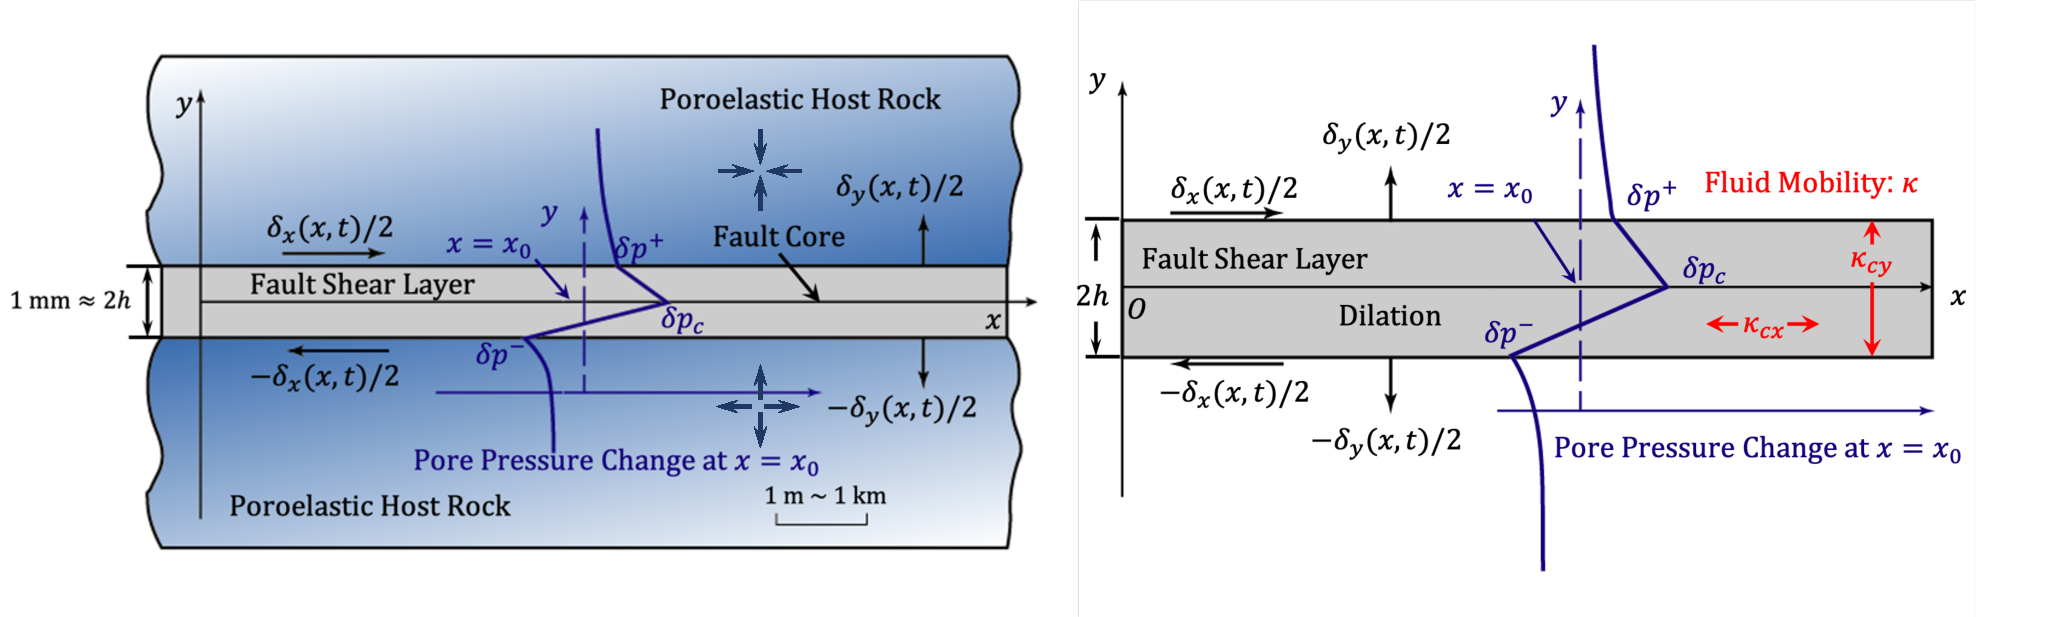
\includegraphics[width=1.0\textwidth]{poroelastic_layer1.pdf}
    \caption{Fault embedded in poroelastic solid medium (left).
    A closer look at the shear layer discussed in the text, with $\delta p_c$ increasing from zero due to fluid injection (right).}
    \label{fig:poroshear1}
\end{figure}

Similarly from the mass conservation of solids in the fault shear layer, 
one can get the control equation on fault opening $\delta_y$ \cite{Elias_Shengduo_2022}.

\begin{align}
    \delta_y &= 2h \left(\frac{\phi_*}{1-\phi_*}\beta_\phi^p-\beta_s^p\right)
    \left(
    \delta p_m - \frac{\frac{\phi_*}{1-\phi_*}\beta_\phi^p+\beta_s^p}{\frac{\phi_*}{1-\phi_*}\beta_\phi^p-\beta_s^p}\sigma
    \right)+\frac{2h\phi^{pl}}{1-\phi_*}, 
    \label{eq:layerControl2}
\end{align}
where $\beta_\phi^p$ and $\beta_s^p$ are compressibility constants. 

Equation (\ref{eq:layerControl1}) and (\ref{eq:layerControl2}) together with Rate-and-State friction forms the control equations of the fault shear layer. 
Then by numerically solving the coupled poroelastic equations for the solid bulk and those control equations for the layer, 
one can study specific fault-slip problems with poroelastic and dilatancy effects.*

For the injector of fluid, 
since in this study we aim to study the effect of injection rate, 
injection-time profile, etc., 
we need a baseline case with the total mass of injected fluid controlled, 
based on which we modify the flux of injection vs. time and examine its effects on the fault slip. 
Motivated by the pressure-control injection in (Elias et al., 2022) \cite{Elias_Shengduo_2022}, 
we take their averaged flux over the experiment window (1400 s), 
and use that as our baseline flux. 
Figure~\ref{fig:FluxControl} shows the comparison between the evolution of pore fluid pressure and slip rate over the fault under pressure-control injection and flux-control injection with the same average flux. 
The material properties which are kept the same in both cases can be found in Table~\ref{tab:elasticBulk} and \ref{tab:fricPropsFault}. 
We find that the flux-control injection case has qualitatively similar response compared with the pressure-control injection, 
while the pore fluid pressures $p^+, p^-$ and $p_c$ increase faster with time upon the start of the injection. 
In the following discussion we will refer to the flux-control case with baseline flux $1\times10^{-4}\ \mathrm{Kg/(m\cdot s)}$ as the baseline case. 

\begin{figure}[htbp]
    \centering
    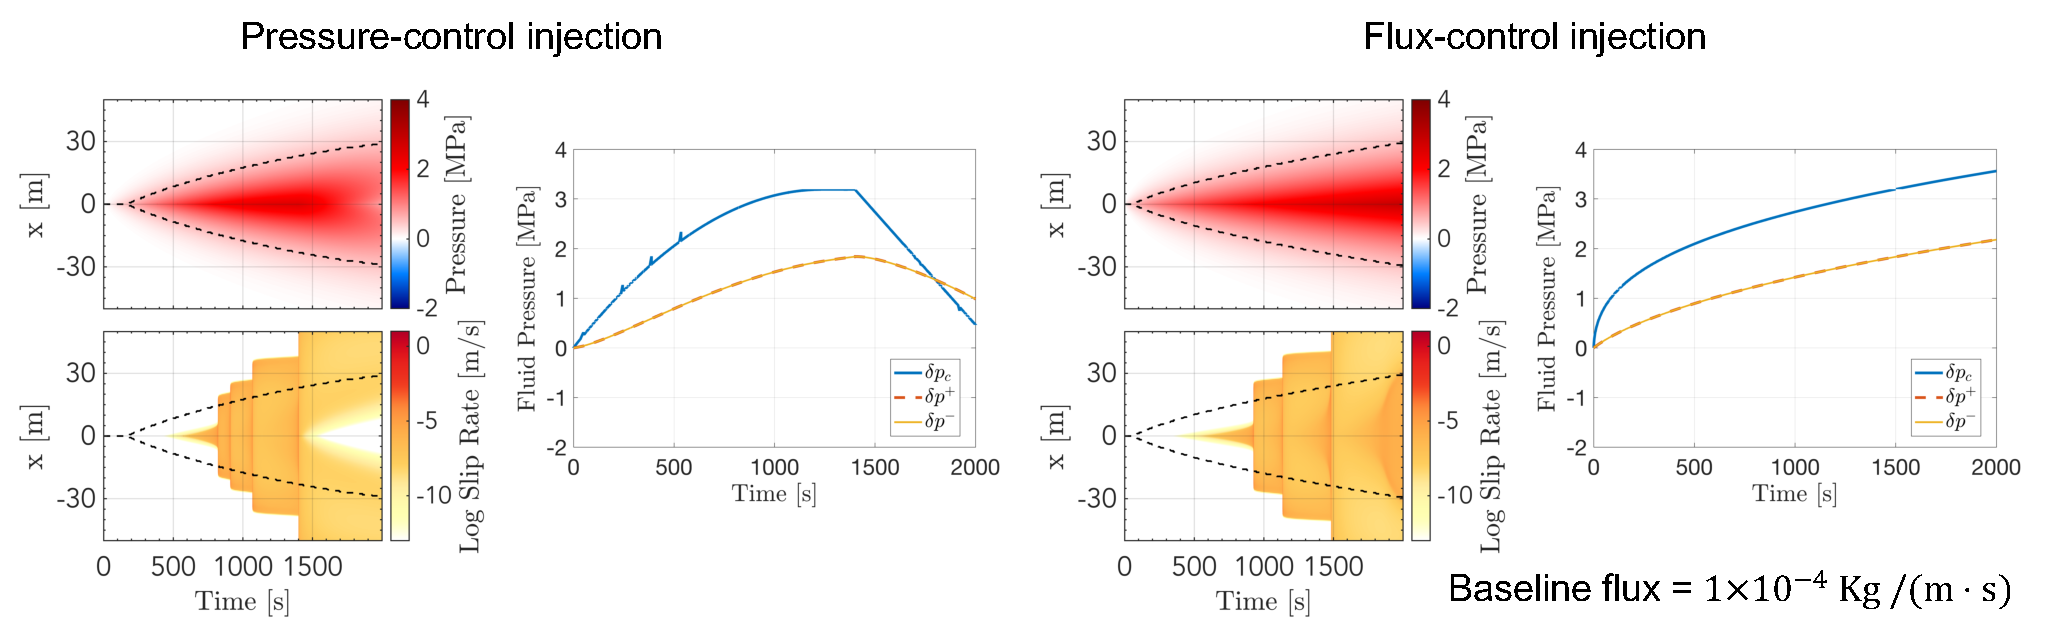
\includegraphics[width=1.0\textwidth]{figures/FluxControl.pdf}
    \caption{Comparison of slip rate and pore pressure evolution under pressure-control injection and flux-control injection. 
    The flux is set to be the average flux in the pressure-control injection case.}
    \label{fig:FluxControl}
\end{figure}